\documentclass{beamer}

\usepackage{color}
%\definecolor{class}{RGB}{111,159,207}
%\definecolor{literal}{rgb}{0.58,0,0.82}

\usepackage{hyperref}
\hypersetup{colorlinks=true, linkcolor=black, citecolor=blue, urlcolor=blue}

\usepackage[absolute,overlay]{textpos}
\TPGrid{100}{100}

\usepackage[ % BIBLATEX
  backend=bibtex,
  style=numeric-comp,sorting=none,block=ragged,firstinits=true
]{biblatex}
\bibliography{tilelvreqs}

\usepackage{tikz}

%\usepackage{forloop}
\usepackage{pdfpages}
\usepackage{pgf}

\usepackage{colortbl}

% Fixes ---------------------------------------------------
%\usepackage{lmodern}
\usepackage{silence}
\WarningFilter{biblatex}{Patching footnotes failed}

\let\Tiny=\tiny

% Slide styles --------------------------------------------
\setbeamersize{text margin left=20px,text margin right=20px}
\setbeamertemplate{navigation symbols}{}
\setbeamertemplate{section in toc}[sections numbered]
\setbeamertemplate{subsubsection in toc}[subsubsections numbered]
\setbeamertemplate{footline}{%
  \usebeamerfont{author in head/foot}%
  \insertshortauthor[width={1.7cm},respectlinebreaks,center]%
  \hspace*{-0.8mm},\ %
  \usebeamerfont{date in head/foot}\insertdate%
  \hspace*{1mm}%
  \usebeamerfont{footline}\url{https://indico.cern.ch/event/467725/}%
  \hfill%
  \insertframenumber/\inserttotalframenumber%
  \hspace*{1mm}
}
\setbeamertemplate{bibliography item}{\insertbiblabel}

\def\changemargin#1#2{\list{}{\rightmargin#2\leftmargin#1}\item[]}
\let\endchangemargin=\endlist

% Title, Authors, Date ************************************
\title{Low Voltage Monitoring Upgrade\\for ATLAS Tile Calorimeter}
\author[Ivan Pogrebnyak]
{%
  \texorpdfstring{
    \centering
    I. Pogrebnyak \\
    Working with: A. Paramonov, G. Drake, J. Proudfoot \\
  }{Ivan Pogrebnyak}
}
\date{December 8, 2015}

%%%%%%%%%%%%%%%%%%%%%%%%%%%%%%%%%%%%%%%%%%%%%%%%%%%%%%%%%%%
\begin{document}

% Title slide ---------------------------------------------
\frame{
  \begin{tikzpicture}[remember picture,overlay]
    \node[anchor=north west] at (current page.north west){
      
\includegraphics[height=30pt]{logos/msu_helmet}
      \vspace{5px}
      
\includegraphics[height=30pt]{logos/msu_text}
    };
    \node[anchor=north east] at (current page.north east){
      \begin{minipage}{100px}
      \vspace{-21px}
      {\huge Argonne}\\
      {\large National Laboratory}
      \end{minipage}
      
\includegraphics[height=30pt]{logos/argonne_logo}
    };
    \node[anchor=south west] at (current page.south west){
      \begin{minipage}{100px}
      
\includegraphics[height=30pt]{logos/DOE_Logo_Color}
      \vspace{8px}
      \end{minipage}
    };
    \node[anchor=south east] at (current page.south east){
      \begin{minipage}{96px}
      {\huge ATLAS}
      \vspace{-21px}\\
      {\large Experiment}
      \hspace{5px}
      
\includegraphics[height=30pt]{logos/cern_logo}
      \vspace{8px}
      \end{minipage}
    };
  \end{tikzpicture}

  \titlepage
}

% TOC -----------------------------------------------------
\frame{\frametitle{Outline}\tableofcontents}

% *********************************************************

\setlength{\leftmargini}{2px}

\section{TileCal hardware and electronics}
\frame{\frametitle{Outline}\tableofcontents[currentsection]}

\frame{\frametitle{TileCal hardware}
  \begin{changemargin}{-20px}{-20px}
    \centering
    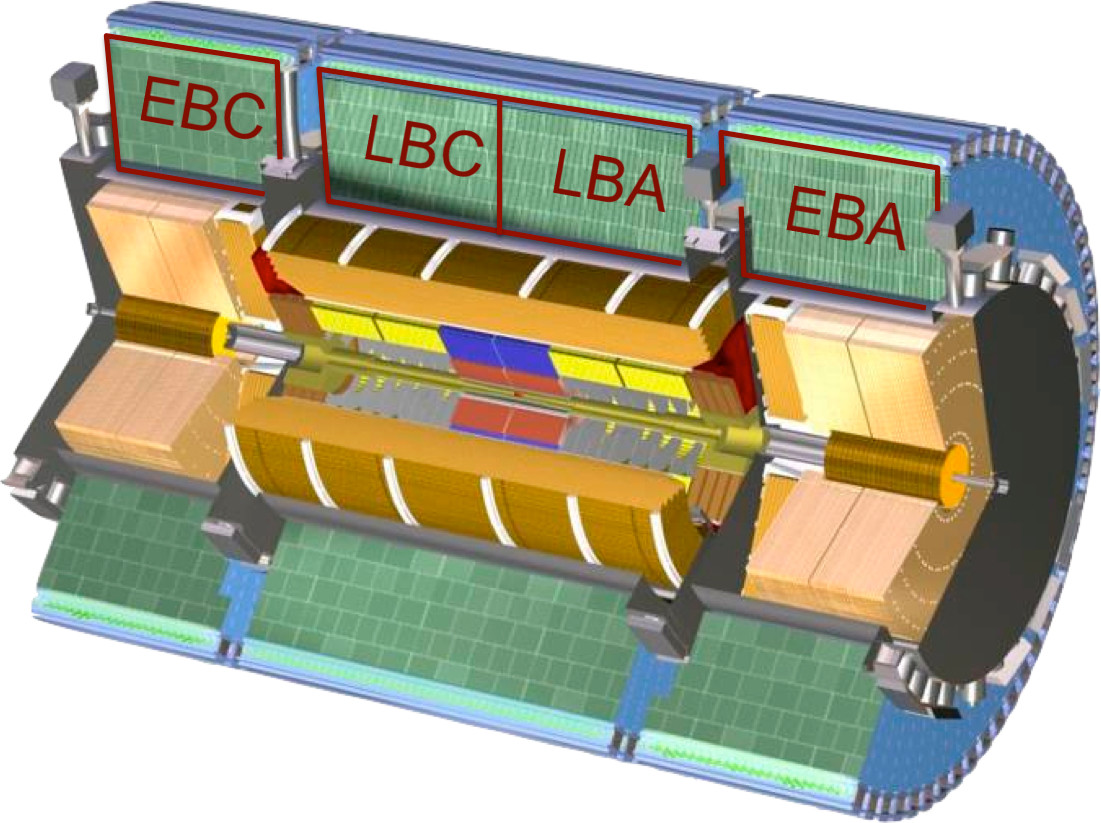
\includegraphics[width=0.9\textwidth]{fig/TileCal_barrels.jpg}
  \end{changemargin}
  \begin{textblock}{30}(7,83)
    LB - Long Barrel\\
    EB - Extended Barrel
  \end{textblock}
  \begin{textblock}{1}(88,90)
    {\tiny Ref.~\cite{twiki.ific}}
  \end{textblock}
}

\frame{\frametitle{TileCal hardware}
  \begin{changemargin}{-20px}{-20px}
    \centering
    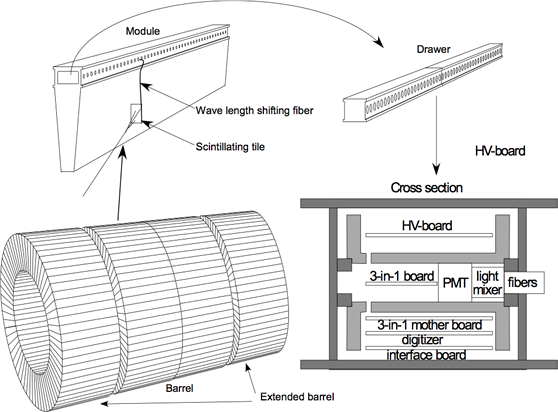
\includegraphics[width=0.9\textwidth]{fig/TileCalMechanicsElectronics}
  \end{changemargin}
  \begin{textblock}{1}(88,90)
    {\tiny Ref.~\cite{uchicago-tile}}
  \end{textblock}
}

\frame{\frametitle{TileCal hardware}
  \begin{changemargin}{-20px}{-20px}
    \centering
    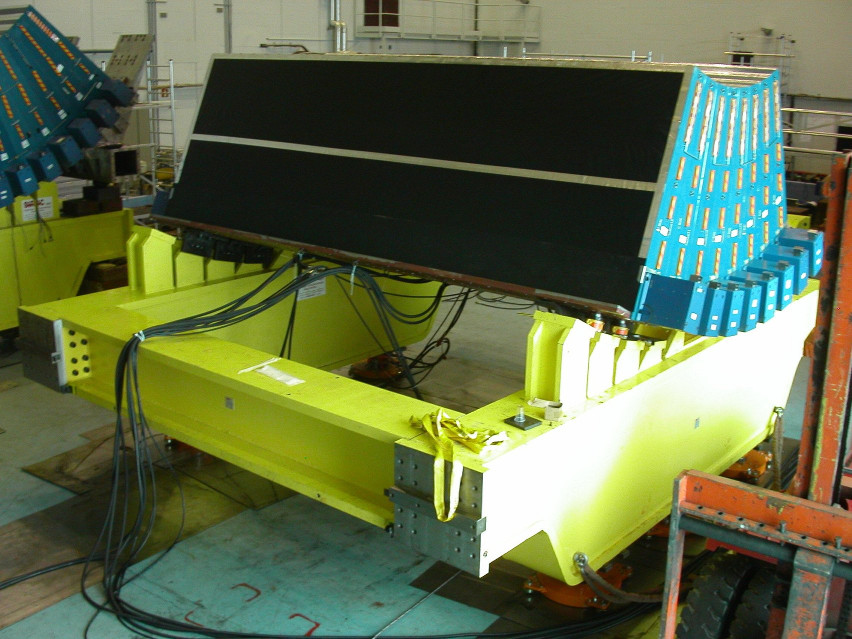
\includegraphics[width=0.9\textwidth]{fig/tilecal-2004-001}
  \end{changemargin}
  \begin{textblock}{20}(57,55)
    
\includegraphics[width=\textwidth]{fig/fLVPS_bubble}
  \end{textblock}
  \begin{textblock}{1}(91,90)
    {\tiny Ref.~\cite{Nemecek:726095}}
  \end{textblock}
}

{
  \addtocounter{framenumber}{1}
  \setbeamercolor{background canvas}{bg=}
  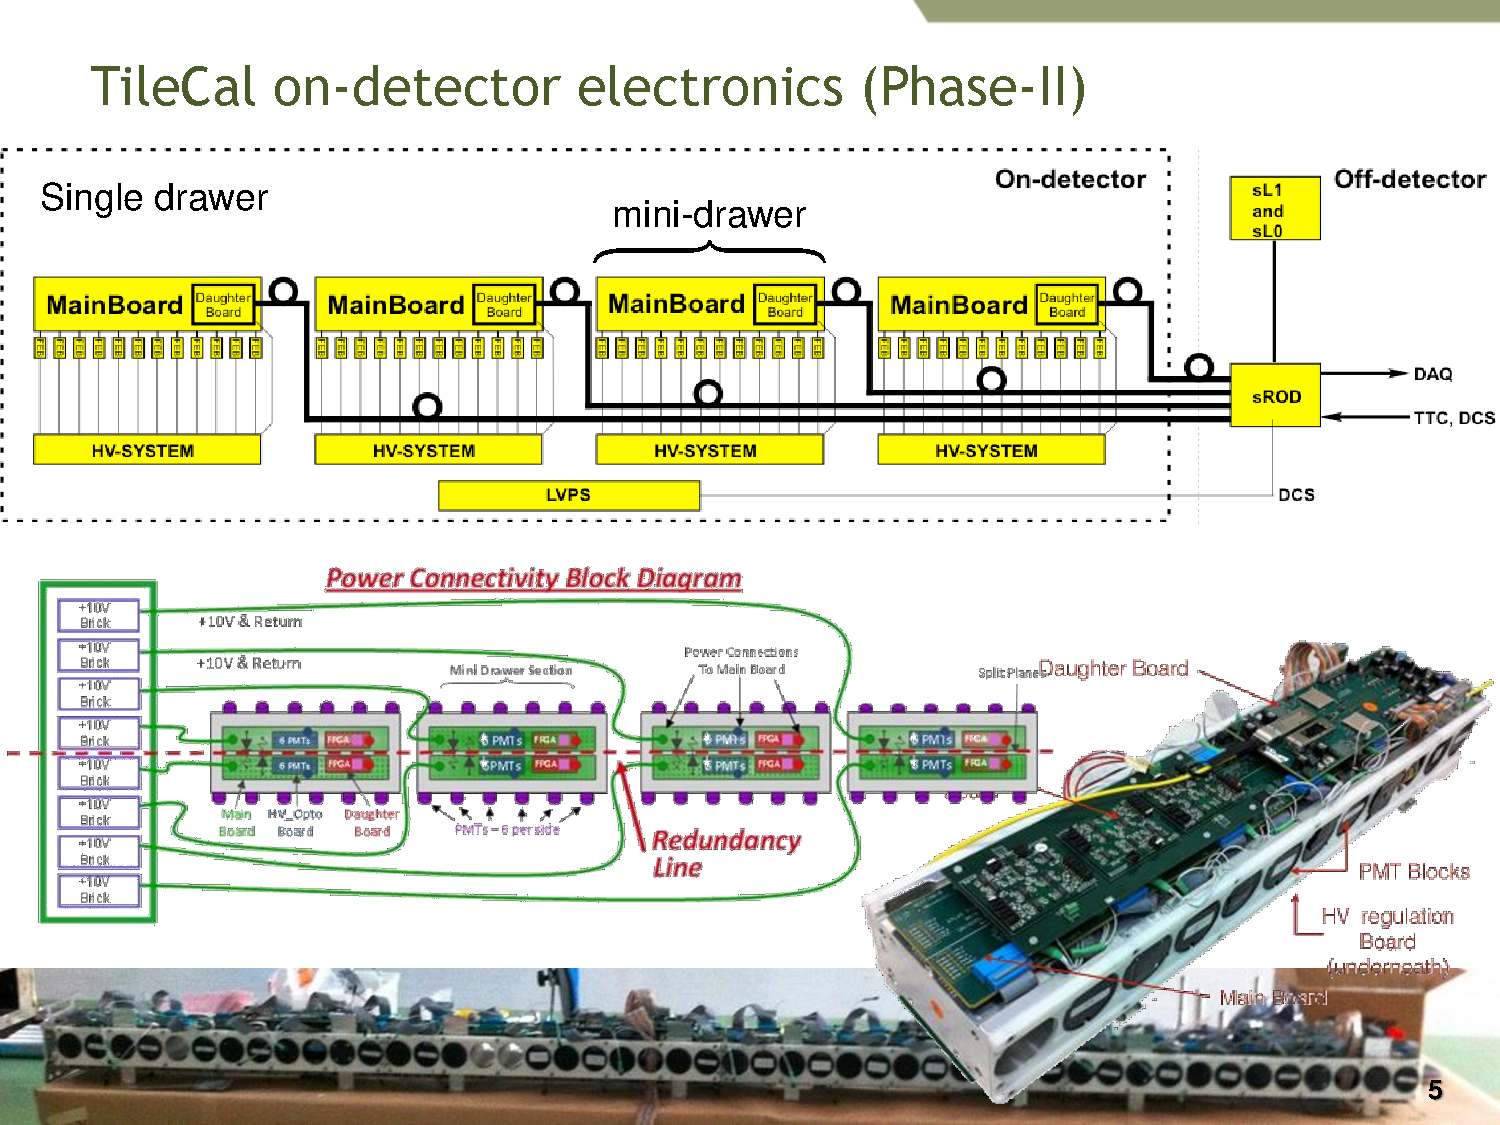
\includepdf[pagecommand={\pagestyle{plain}}]{slides/us_atlas.pdf}
}

{
  \addtocounter{framenumber}{1}
  \setbeamercolor{background canvas}{bg=}
  \begin{textblock}{100}(2.5,4)
    {\usebeamercolor[fg]{title}\usebeamerfont{title}
      Phase-I Low Voltage distribution system}
  \end{textblock}
  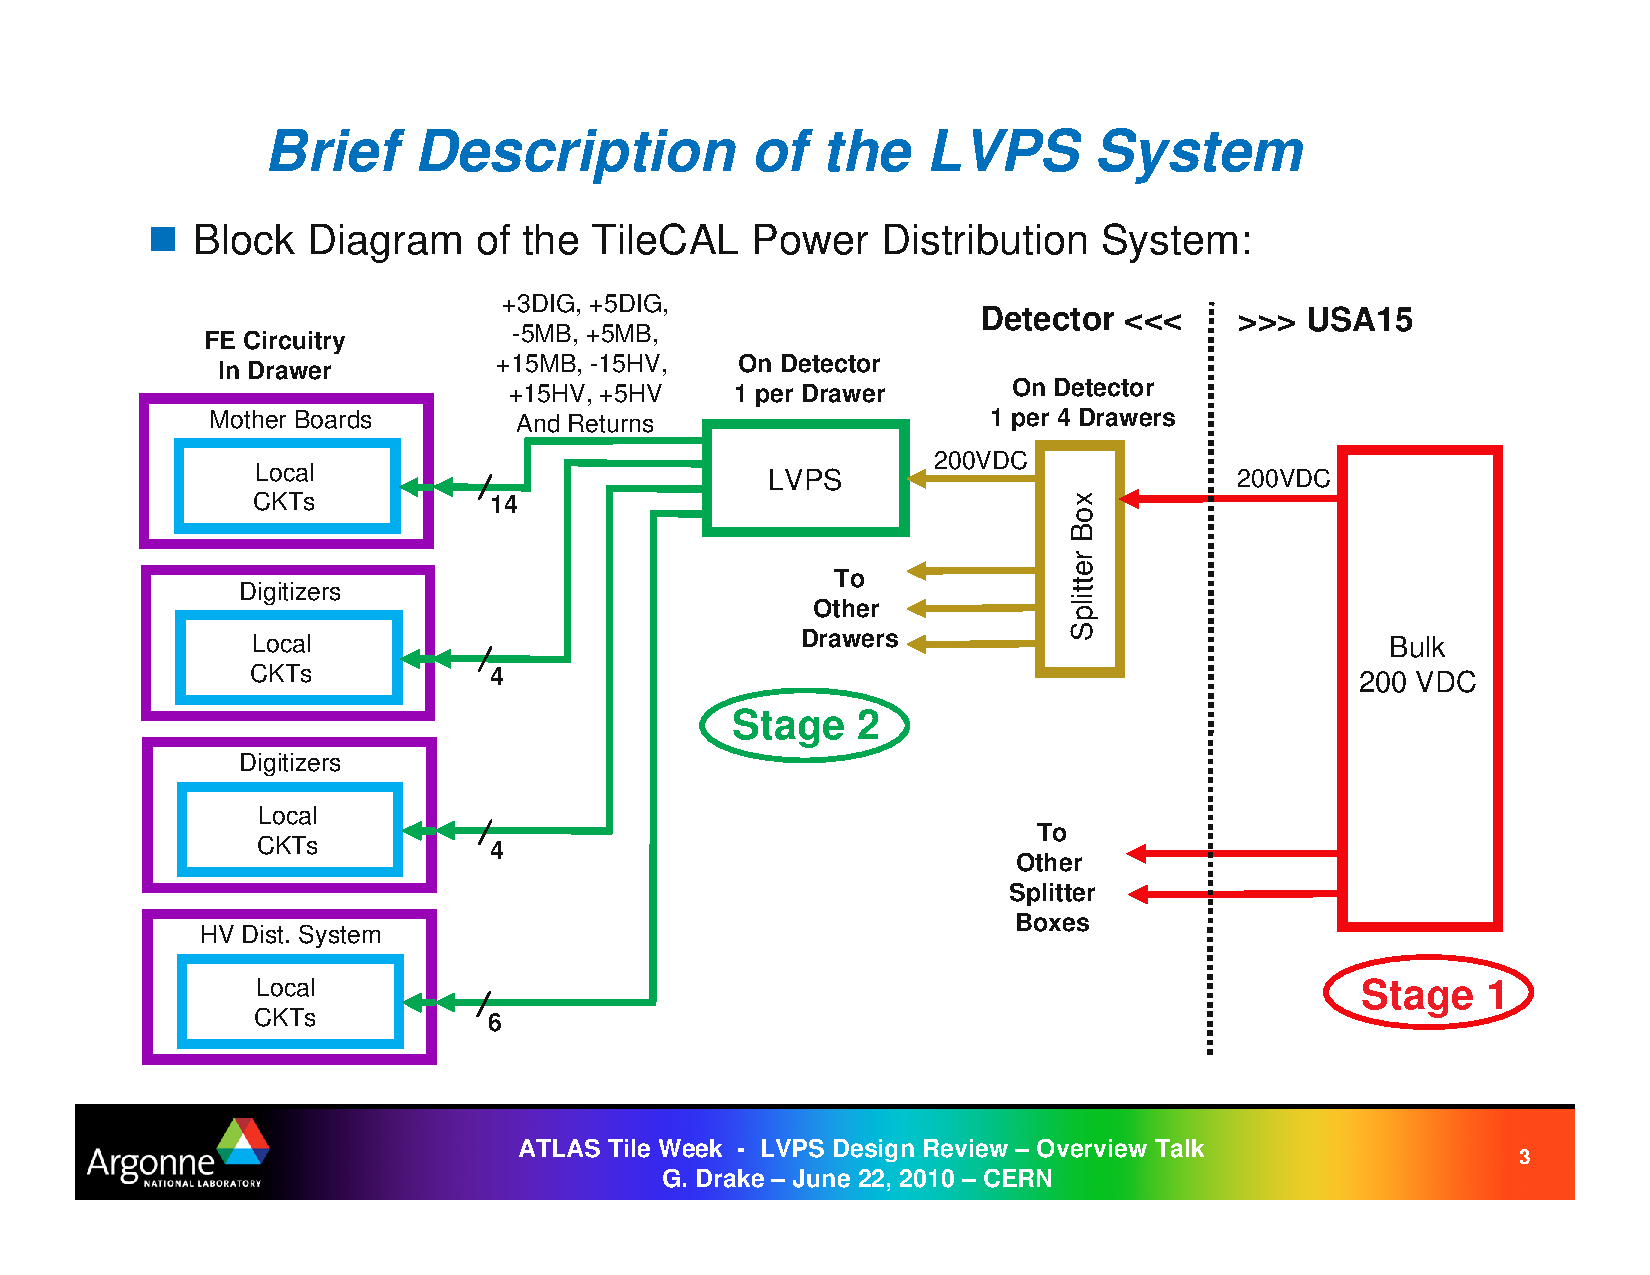
\includepdf[pages=1,pagecommand={\pagestyle{plain}}]{slides/gary.pdf}
}{
  \addtocounter{framenumber}{1}
  \setbeamercolor{background canvas}{bg=}
  \begin{textblock}{100}(2.5,4)
    {\usebeamercolor[fg]{title}\usebeamerfont{title}
      Phase-I Low Voltage distribution system}
  \end{textblock}
  \includepdf[pages=2,pagecommand={\pagestyle{plain}}]{slides/gary.pdf}
}{
  \addtocounter{framenumber}{1}
  \setbeamercolor{background canvas}{bg=}
  \begin{textblock}{100}(2.5,4)
    {\usebeamercolor[fg]{title}\usebeamerfont{title}
      Phase-I Low Voltage distribution system}
  \end{textblock}
  \includepdf[pages=3,pagecommand={\pagestyle{plain}}]{slides/gary.pdf}
}{
  \addtocounter{framenumber}{1}
  \setbeamercolor{background canvas}{bg=}
  \begin{textblock}{100}(2.5,4)
    {\usebeamercolor[fg]{title}\usebeamerfont{title}
      Phase-I Low Voltage distribution system}
  \end{textblock}
  \includepdf[pages=4,pagecommand={\pagestyle{plain}}]{slides/gary.pdf}
}{
  \addtocounter{framenumber}{1}
  \setbeamercolor{background canvas}{bg=}
  \begin{textblock}{100}(2.5,4)
    {\usebeamercolor[fg]{title}\usebeamerfont{title}
      Phase-I Low Voltage distribution system}
  \end{textblock}
  \includepdf[pages=5,pagecommand={\pagestyle{plain}}]{slides/gary.pdf}
}{
  \addtocounter{framenumber}{1}
  \setbeamercolor{background canvas}{bg=}
  \begin{textblock}{100}(2.5,4)
    {\usebeamercolor[fg]{title}\usebeamerfont{title}
      Phase-I Low Voltage distribution system}
  \end{textblock}
  \includepdf[pages=6,pagecommand={\pagestyle{plain}}]{slides/gary.pdf}
}

\frame{\frametitle{fLVPS photos}
  \begin{textblock}{55}(45,0)
    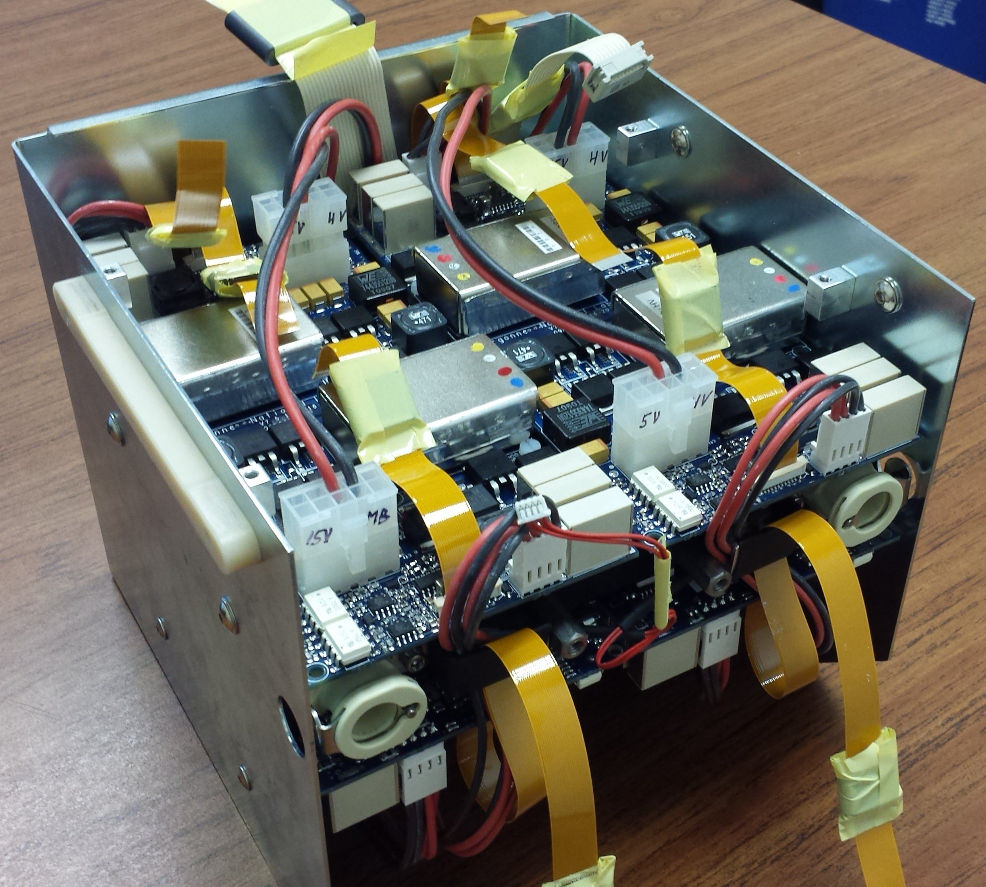
\includegraphics[width=\textwidth]{fig/lvps_bricks}
  \end{textblock}
  \begin{textblock}{60}(0,29)
    \pgfdeclaremask{elmb_mask}{fig/lvps_with_elmb_mask.jpg}
    \pgfimage[width=\textwidth, mask=elmb_mask]{fig/lvps_with_elmb}
  \end{textblock}
}

%**********************************************************

\section{LVPS monitoring problem}
\frame{\frametitle{Outline}\tableofcontents[currentsection]}

\frame{\frametitle{LVPS trips and monitoring problem}
  \begin{itemize}
    \item Constant LVPS trips plagued TileCal operation in Run 1.
    \begin{itemize}
      \item Most trip could be recovered from by power-cycling.
      \item Some could not be fixed without opening the detector.
    \end{itemize}
    \vspace{5mm}
    \item Trips' cause could only be diagnosed during shutdown.
    \vspace{5mm}
    \item Slow monitoring information collected by ELMB was not sufficient to identified failed subsystem.
  \end{itemize}
}

\frame{\frametitle{The problem with trips has been addressed}
  \begin{itemize}
    \item The original designed of LVPS brick from Prague proved to have
          design flaws.%~\cite{REF}.
    \vspace{5mm}
    \item Gary Drake worked on a new LVPS design, which eliminated most
          trips.%~\cite{REF}.
    \vspace{5mm}
    \item But the monitoring problem still remains.
    \begin{itemize}
      \item Currently, it is still not possible to identify the cause of
            an on-detector electronics failure on-line.
    \end{itemize}
  \end{itemize}
}

\frame{\frametitle{Addressing the monitoring problem}
  \begin{itemize}
    \item But the monitoring problem still remains.
    \item Addressing it is the goal of my project.
    \item Currently, it is still not possible to identify the cause of
          an on-detector electronics failure on-line.
    \item We considered the possibility of improving the monitoring system
          for the near future.
    \item Unfortunately, we found it not feasible to make improvements
          before the Phase-II upgrade.
    \item However, improvements can be made.
    \item We found that LVPS brick output current transient can be used
          as a discriminant between types of failure.
  \end{itemize}
}

{
  \addtocounter{framenumber}{1}
  \setbeamercolor{background canvas}{bg=}
  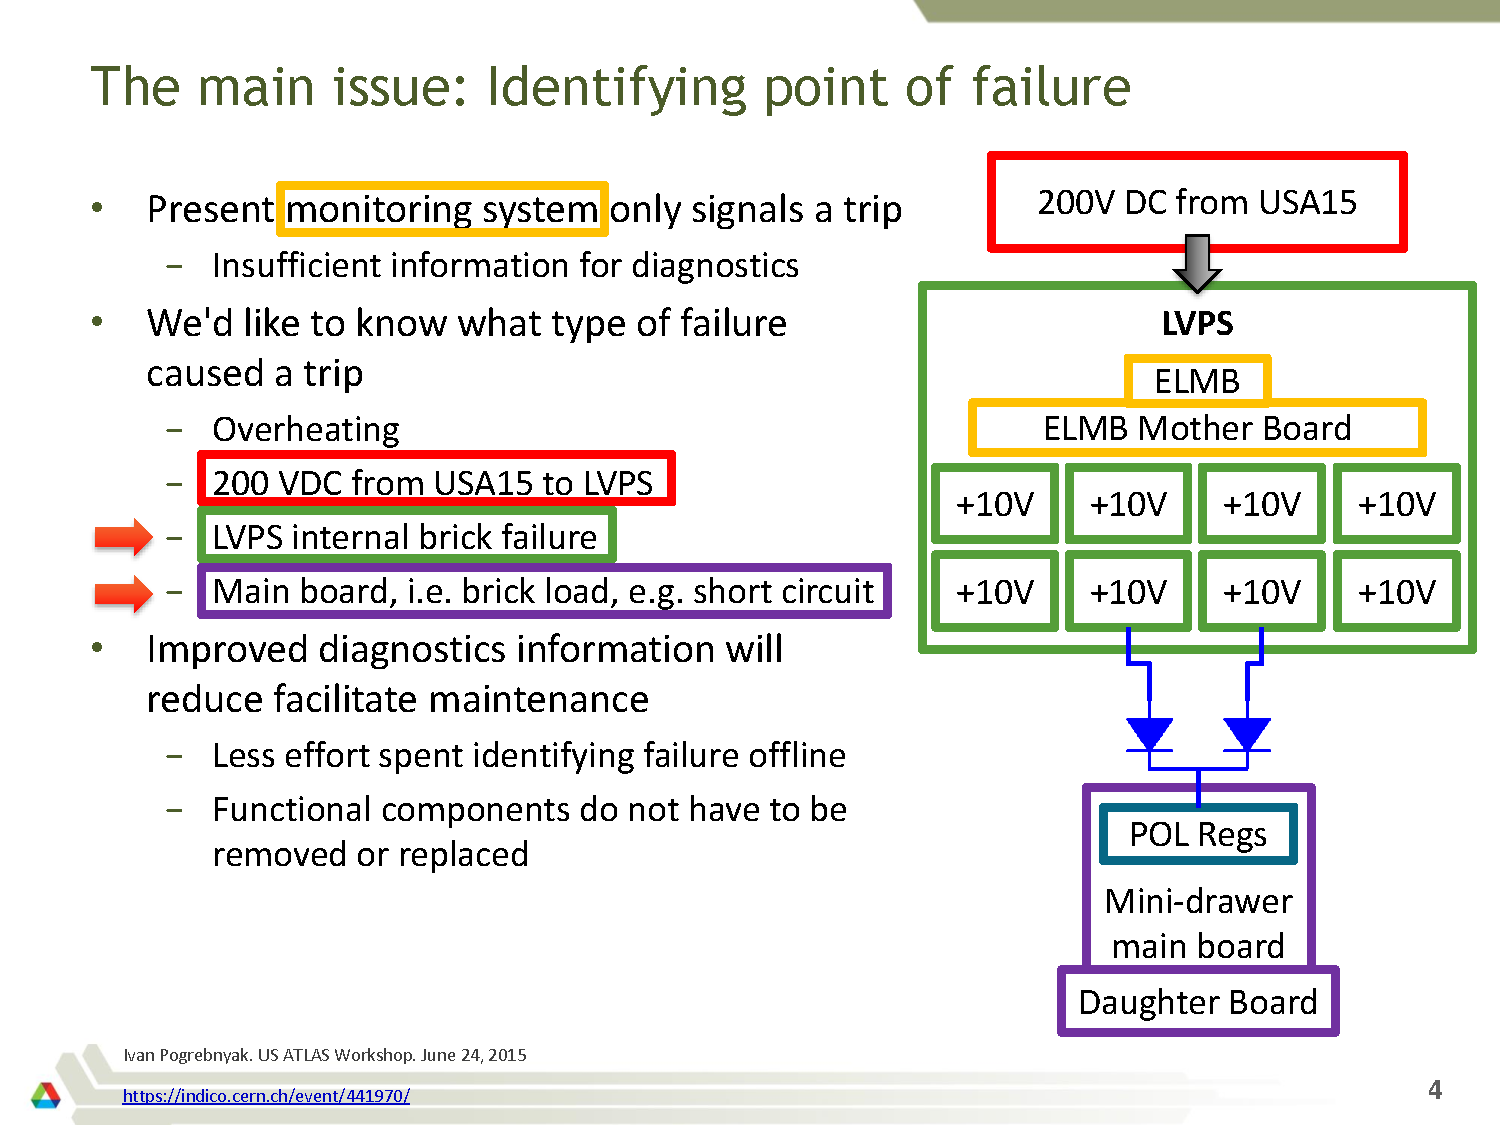
\includepdf[pagecommand={\pagestyle{plain}}]{slides/main_issue}
}

\frame{\frametitle{ELMB128 and its limitations}
  \begin{itemize}
    \item The main problem is sampling frequency.
  \end{itemize}
  \begin{changemargin}{-20px}{-20px}
    \centering
    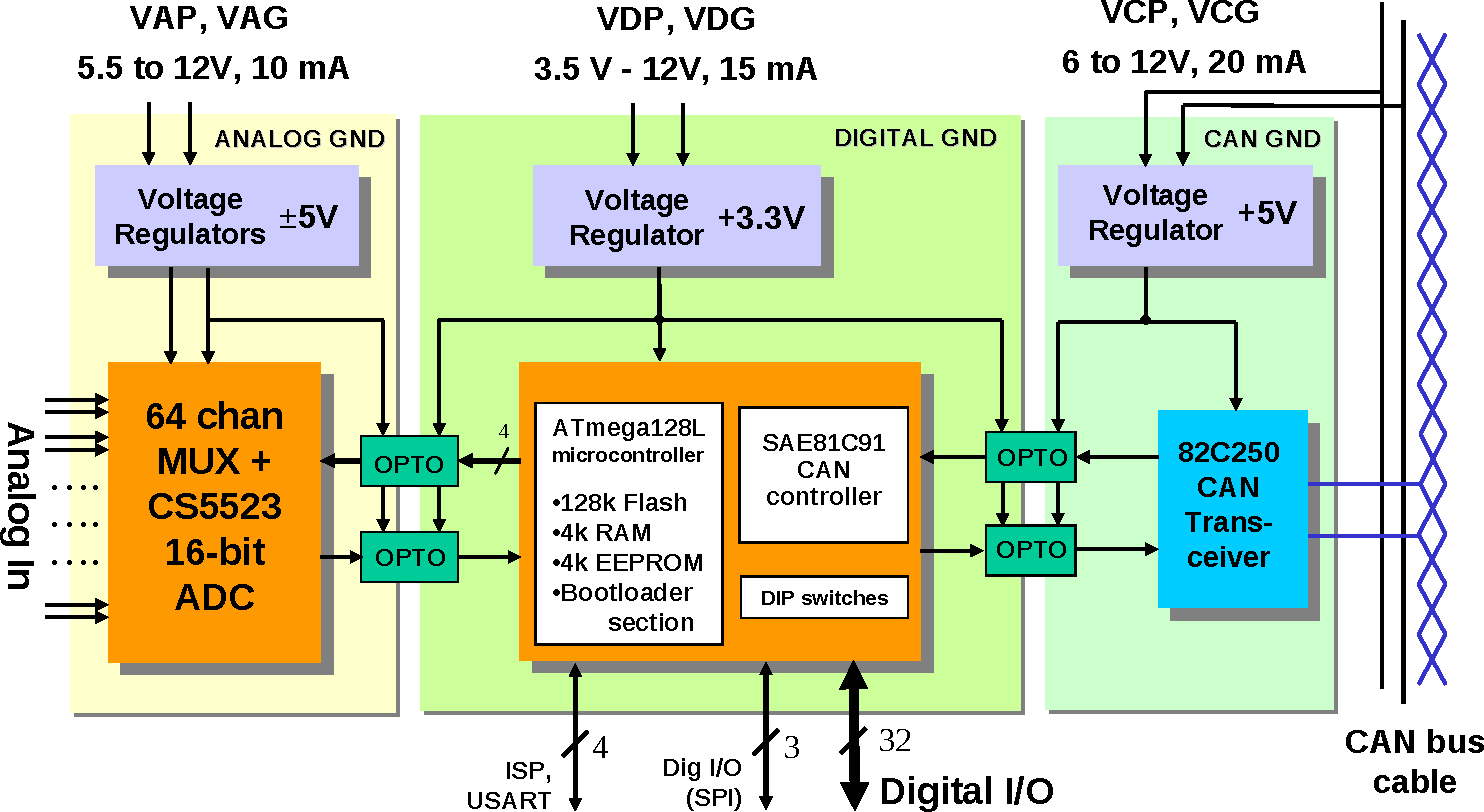
\includegraphics[height=130pt]{fig/elmb_block}
    \hspace{5px}
    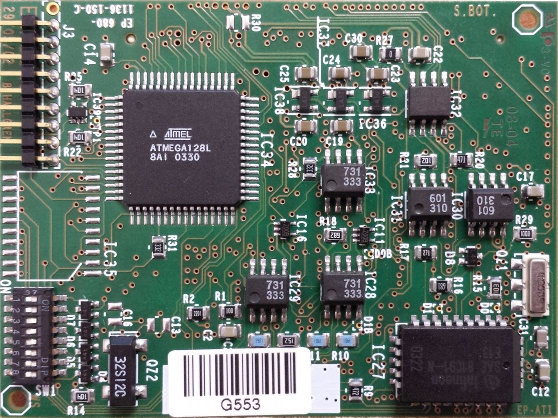
\includegraphics[height=75pt]{fig/elmb_photo}
  \end{changemargin}

  {\centering\scriptsize
  \begin{tabular}{p{40mm}|p{66mm}}
    \hline
    Component & Limitation \\
    \hline
    \hline
    \href{http://www.cirrus.com/en/pubs/proDatasheet/CS5521-22-23-24-28_F8.pdf}{CS5523} ADC
    & Nominal maximum digitization rate of 600 Hz \\
    \href{http://www.pericom.com/assets/Datasheets/107.pdf}{32S12C} 32.768 kHz ADC crystal
    & Limits the ADC maximum digitization rate to 101 Hz \\
    \href{http://www.farnell.com/datasheets/1524140.pdf}{HCPL0731}
      optocoupler between the analog and digital stages
    & Limits the ADC maximum digitization rate to 30 Hz \\
    \href{http://www.atmel.com/devices/atmega128.aspx}{Atmega128L} microcontroller
    & Allows for local storage of only one value per channel \\
    \hline
  \end{tabular}
  }
}

%**********************************************************

\section{Use of transients for trip diagnostics}
\frame{\frametitle{Outline}\tableofcontents[currentsection]}

\frame{\frametitle{Use of transients for trip diagnostics}
  \begin{changemargin}{-20px}{-20px}
    \centering
    % trim=left bottom right top
    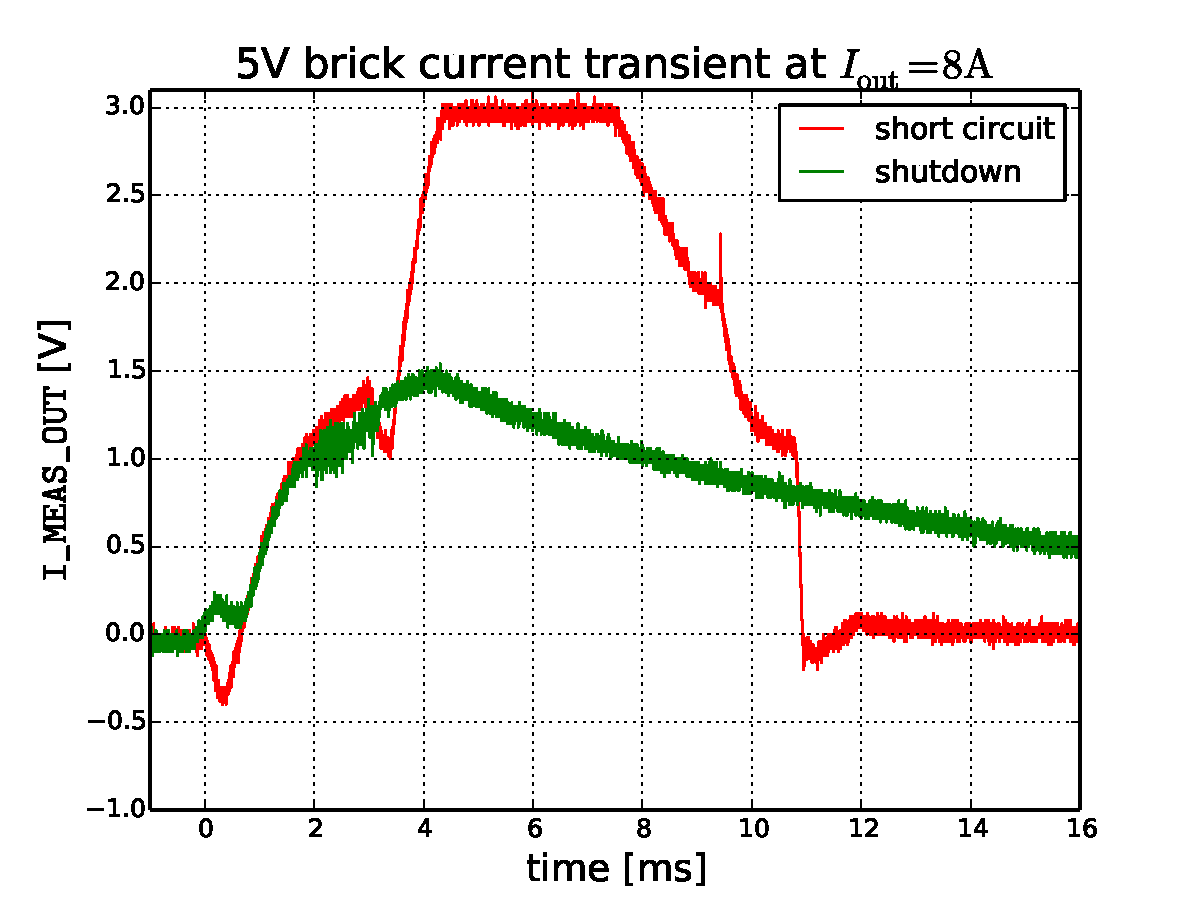
\includegraphics[height=140pt,trim=10px 6px 50px 10px,clip]{fig/current}
    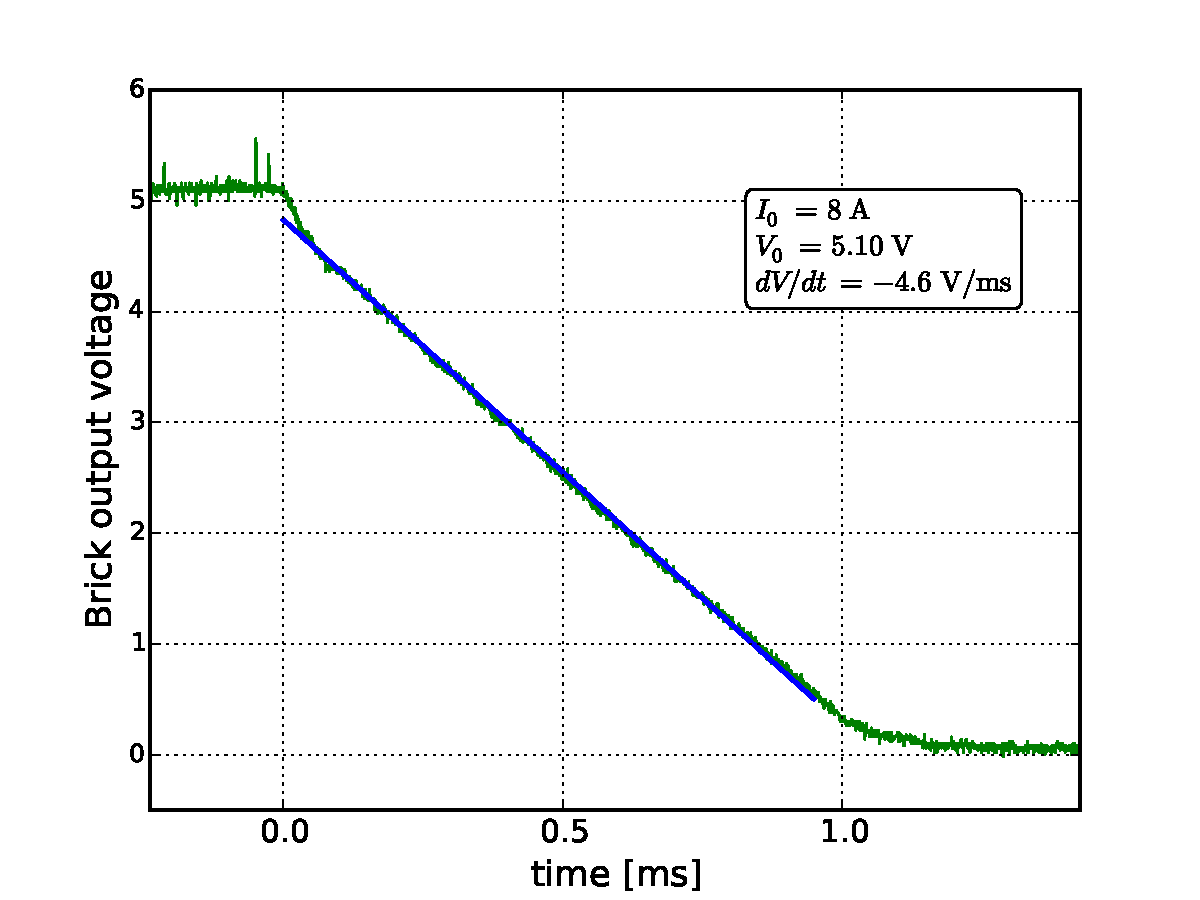
\includegraphics[height=140pt,trim=10px 6px 50px 10px,clip]{fig/direct_Vout}
  \end{changemargin}
  {\scriptsize
  \begin{itemize}
    \item The current reaches the over-current threshold when the brick is overloaded ({\color{red}red line}).
    \item The current does not rise to the same level when a brick experiences
          an internal failure or a shut down ({\color[HTML]{008000}green line}).
    \item The information is sufficient to diagnose the cause of the trip.
    \item The shape of the pulse depends on the parameters of the filter circuit.
    \item Output voltage decays linearly because active load, used at the test bench,
          adjusts impedance to consume constant current.
  \end{itemize}
  }
}

\frame{\frametitle{LVPS brick monitoring filter}
  \begin{changemargin}{-20px}{-20px}
    \centering
    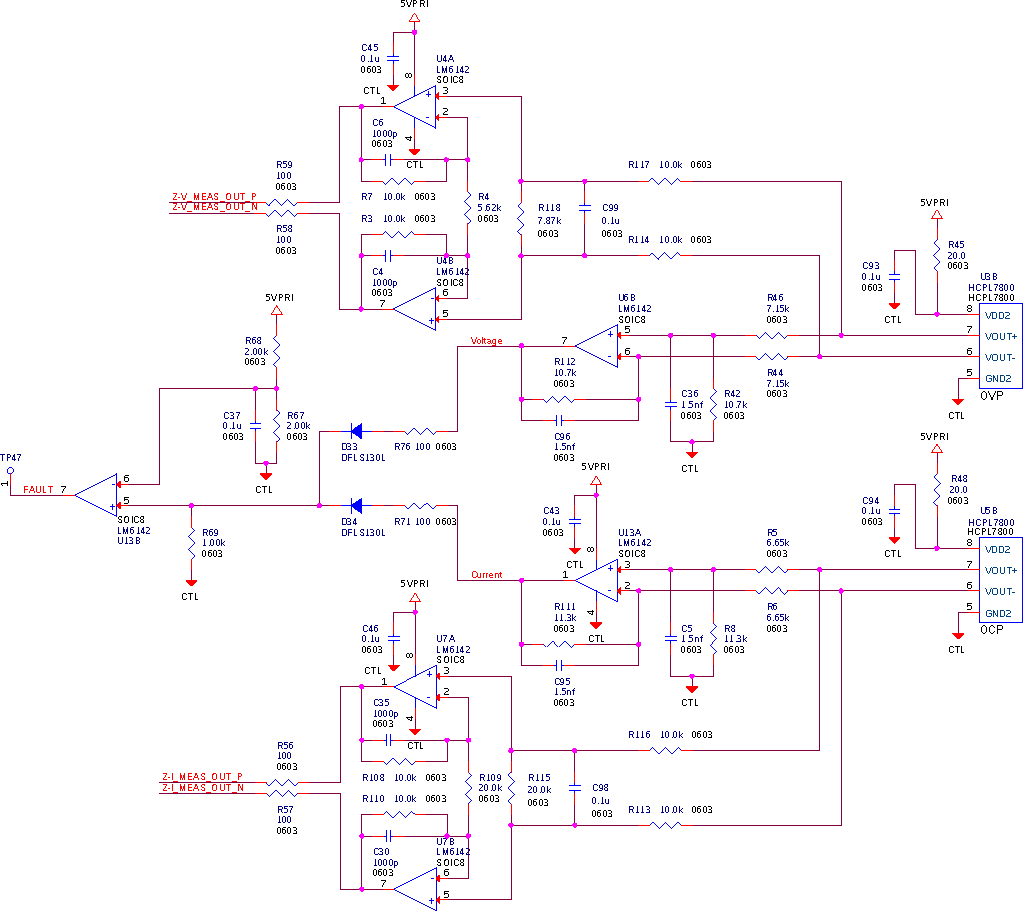
\includegraphics[height=240pt]{fig/filter}
  \end{changemargin}
}

\frame{\frametitle{10V brick transients}
  \begin{changemargin}{-20px}{-20px}
    \centering
    % trim=left bottom right top
    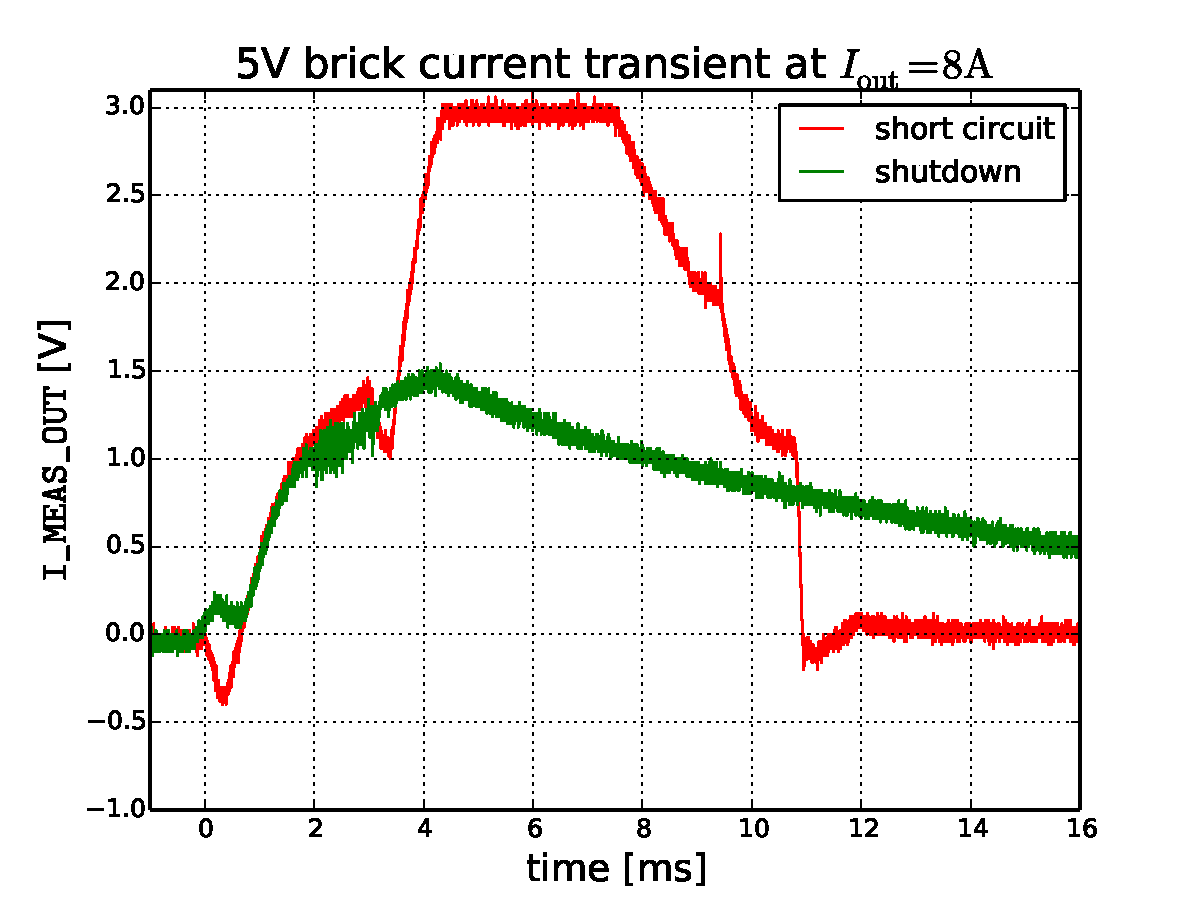
\includegraphics[height=140pt,trim=10px 6px 50px 10px,clip]{fig/current}
    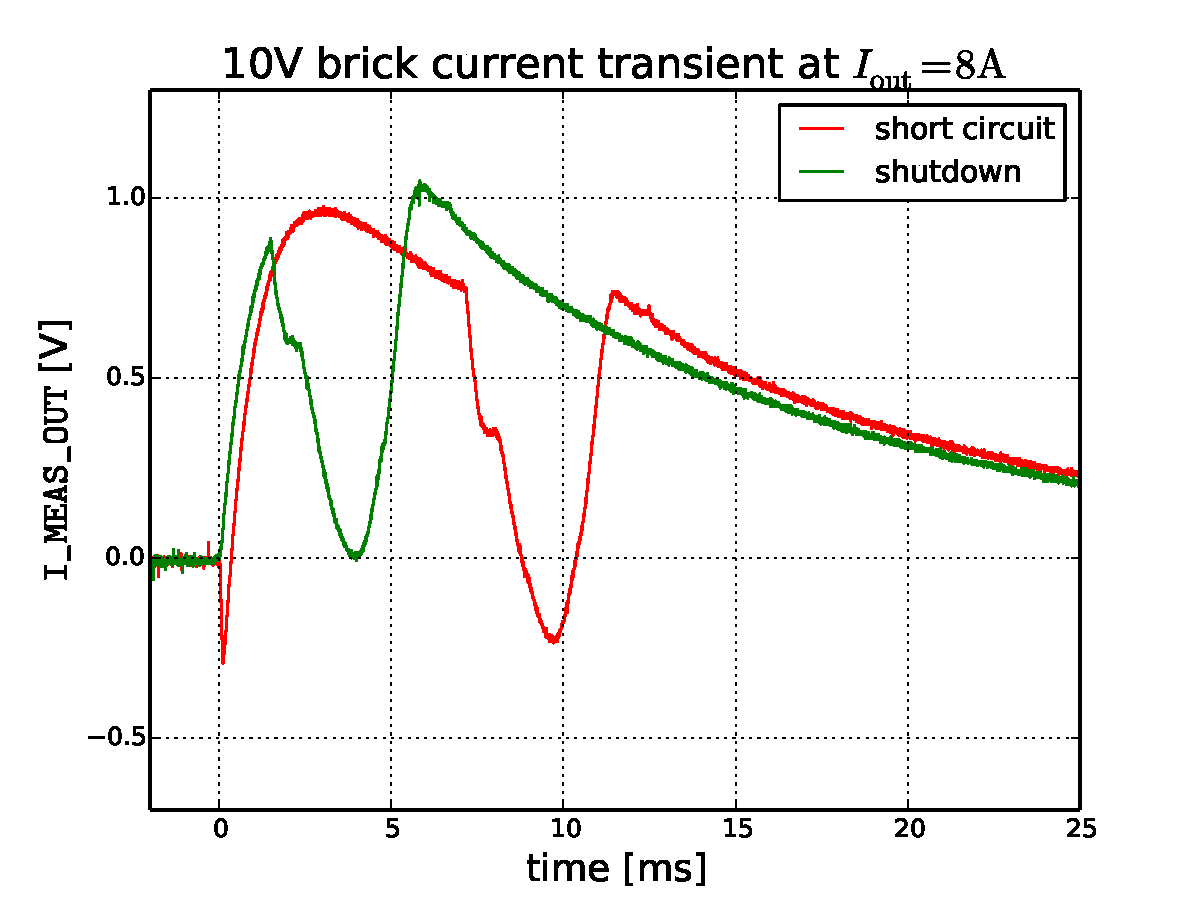
\includegraphics[height=140pt,trim=10px 6px 50px 10px,clip]{fig/current_10V}
  \end{changemargin}
  \begin{itemize}
    \item Purely an artifact of the filter circuit.
    \item Common features are visible.
    \item Adjustment of RC components should mitigate this effect.
  \end{itemize}
}

%**********************************************************

\section{Requirements for Phase-II upgrade}
\frame{\frametitle{Outline}\tableofcontents[currentsection]}

\frame{\frametitle{Requirements for LVPS bricks}
  \begin{itemize}
    \item Tune brick signal filter circuits to improve
          differentiability between load short circuit and internal failure
          trips.
    \begin{itemize}
      \item May be as trivial as adjusting RC components
    \end{itemize}
    \vspace{10mm}
    \item If the rise in current transient for internal failure trip can be
          sufficiently reduced, failure type identification may be
          simplified to a threshold condition for peak of the transient.
  \end{itemize}
}

\frame{\frametitle{Wishlist for the ELMB++ (hardware)}
  \begin{itemize}
    \item {\bf 2 ksps monitoring rate} for every brick output current
    \begin{itemize}
      \item Other parameters can be monitored at a much slower rate
      \item Higher then 500 sps, because changes in filter circuit may shrink transients.
      \item Due to output capacitance, brick transients cannot be shorter then 1 ms.
    \end{itemize}
    \item {\bf On-board memory} to store last 10 output current measurements
    \item {\bf ``Black box" memory} to store last 10 measurements prior to a trip
    \begin{itemize}
      \item Rewritable only after successfully copied to DCS
    \end{itemize}
    \item Store last reported to DCS value for every parameter.
    \item {\bf External ELMB power} to allow continued monitoring in case any or all
    bricks trip
    \item {\bf 10 bit ADC} is sufficient (ELMB128 uses 16 bit ADC)
    \item Must have {\bf comparable size}
  \end{itemize}
}

\frame{\frametitle{Wishlist for the ELMB++ (firmware)}
  \begin{itemize}
    \item {\it In-situ} trip type identification
    \item Push alarms to DCS
    \item Under normal operation, send updated values to DCS only if
    \begin{itemize}
      \item Change sufficiently from previously reported
      \item Cross warning threshold
      \item Have not reported in long time
    \end{itemize}
    \item Monitoring algorithm must allow to detect simultaneous trips
    \item Present CANbus speed should suffice (125 kbit/s)
    \begin{itemize}
      \item Under normal operating mainly send infrequent updates on operating
            parameters
      \item In case of trip, relevant measurements can be retrieved from black box
            memory
    \end{itemize}
  \end{itemize}
}

\frame{\frametitle{Requirements for the ELMB++ Mother Board}
  \begin{itemize}
    \item Provide digital signals for individual brick power-cycling
    \begin{itemize}
      \item No more group shutdown, bricks operate independently
    \end{itemize}
    \vspace{10mm}
    \item Will have to be updated for ELMB++ anyway
  \end{itemize}
}

\definecolor{Green}{HTML}{92D050}
\definecolor{Yellow}{HTML}{FFC000}
\definecolor{Blue}{HTML}{31859C}

\frame{\frametitle{Radiation tolerance requirements}
  {\centering
  \small
  Comparison of simulated and measured quantities of radiation exposure scaled to $3~\mathsf{ab}^{-1}$ integrated luminosity at 14 TeV. Safety factors are not included.
  \tiny
  \begin{tabular}{%
  |c%
  |>{\columncolor{Yellow}}c|>{\columncolor{Yellow}}c%
  |>{\columncolor{Green}}c|>{\columncolor{Green}}c%
  |>{\columncolor{Blue}}c|}
  \hline
  \rowcolor[gray]{0.8}
   & Simulation & RadMon measured & Simulation & RadMon measured & Simulation \\
  \rowcolor[gray]{0.8}
  Region
  & TID $[\mathsf{rad}]$ & TID $[\mathsf{rad}]$
  & NIEL $[\mathsf{cm}^{-2}]$ & NIEL $[\mathsf{cm}^{-2}]$
  & SEE $[\mathsf{cm}^{-2}]$ \\
  \hline
  Tile Daughter Board &
  $1.31\times 10^{2}$ &
   &
  $2.26\times 10^{11}$ &
   &
  $1.71\times 10^{10}$ \\
  \hline
  Tile barrel finger &
  $6.33\times 10^{3}$ &
  0.6 -- 4.4 $\times 10^3$ &
  $1.61\times 10^{12}$ &
  1.8 -- 5.1 $\times 10^{12}$ &
  $3.40\times 10^{11}$ \\
  \hline
  Tile endcap &
  $1.01\times 10^{3}$ &
   &
  $1.39\times 10^{11}$ &
   &
  $3.83\times 10^{10}$ \\
  \hline
  \end{tabular}
  }
}

\frame{\frametitle{Requirements for DCS}
  \begin{itemize}
    \item Incorporate the new mode of communication with ELMB++
    \item Take appropriate actions for different failure types
  \end{itemize}

  {\centering\small
  \begin{tabular}{p{30mm}|p{76mm}}
    \hline
    Trip type & Action \\
    \hline
    \hline
    200V lost
    & Turn on brick when 200V is on \\
    Internal brick failure
    & Attempt to power-cycle \\
    Brick over-voltage
    & Attempt to power-cycle \\
    Brick over-current
    & Attempt to power-cycle only if the backup brick is functioning \\
    Over-temperature
    & Attempt to power-cycle only after temperature decreases \\
    \hline
  \end{tabular}
  }
}

\frame{\frametitle{Internal note draft on CDS}
  \url{https://cds.cern.ch/record/2055254}
  \begin{changemargin}{-20px}{-20px}
    \centering
    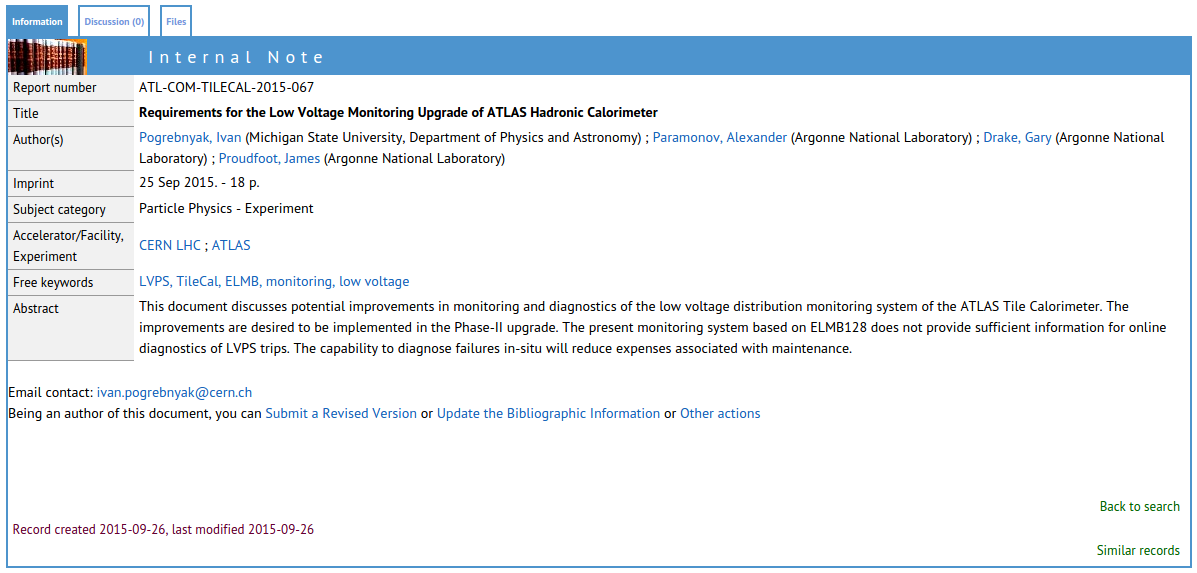
\includegraphics[width=\linewidth]{fig/cds}
  \end{changemargin}
}

%**********************************************************

\section{Alternative solution using GBT-SCA}
\frame{\frametitle{Outline}\tableofcontents[currentsection]}

\frame{\frametitle{GBT-SCA alternative}
  \begin{changemargin}{-20px}{-20px}
    \centering
    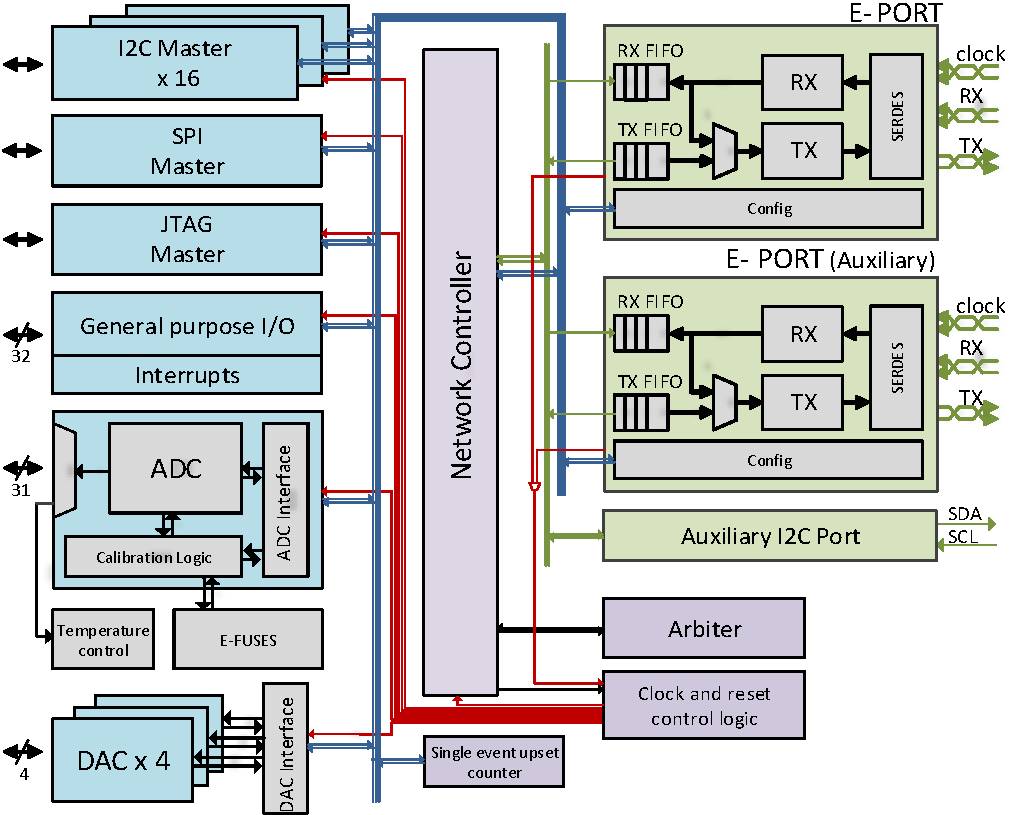
\includegraphics[height=140pt]{fig/gbt-sca_asic}
    \hspace{5px}
    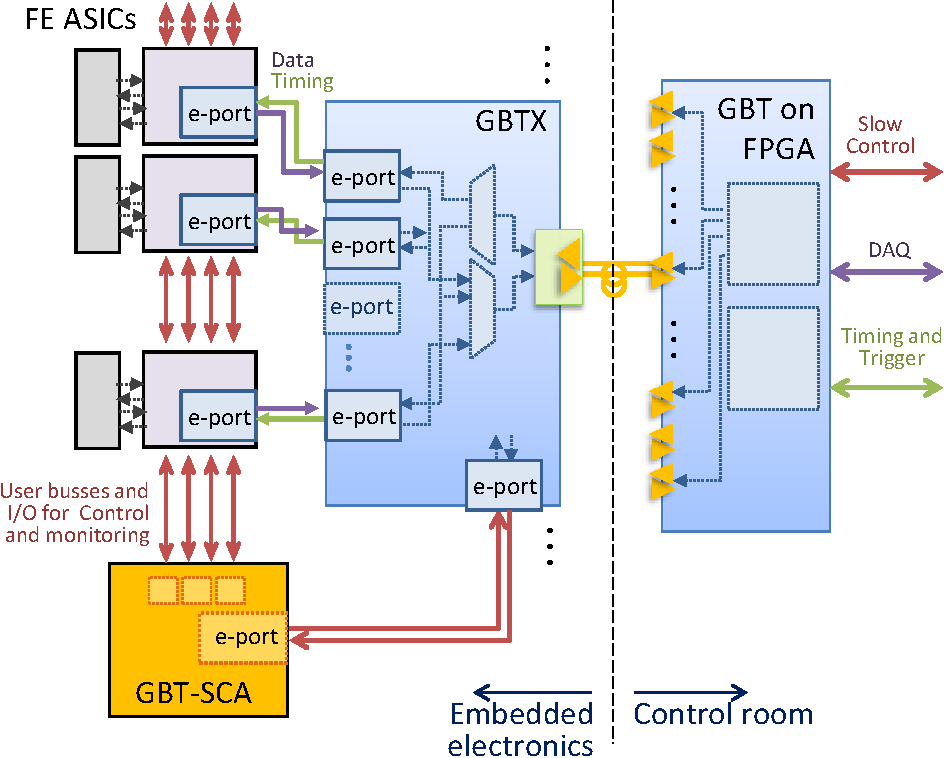
\includegraphics[height=140pt]{fig/gbt-sca_intercon}
  \end{changemargin}
  \begin{textblock}{10}(111,111)
  \cite{cook05,henk11,henk03,giorgi12,sergei11,xadc,doc128,Usai:2026593,lvps_web,gary_lvps,gary_lvps_cds,hruska_brick,elmb_wiki,ATL-DAQ-2003-053,1748-0221-10-03-C03034,GBT-SCA-Manual6,GBT-SCA-Manual7}
  \end{textblock}
}

% Acknowledgements ----------------------------------------
\frame{\frametitle{Acknowledgements}
This material is based upon work at the Argonne National Laboratory supported by the U.S. Department of Energy, Office of Science,
Office of Workforce Development for Teachers and Scientists, Office of Science Graduate Student Research
(SCGSR) program. The SCGSR program is administered by the Oak Ridge Institute for Science and Education for
the DOE under contract number DE-AC05-06OR23100.
}

% BIBLIOGRAPHY --------------------------------------------
\begin{frame}[allowframebreaks]{Bibliography}% in case more than 1 slide needed
  \renewcommand*{\bibfont}{\tiny}
  \printbibliography
\end{frame}

\end{document}
